%%%%% Document Setup %%%%%%%%

\documentclass[12pt, twocolumn]{revtex4}    % Font size (12pt) and column number (one or two).

\usepackage{times}  % Times New Roman font type

\usepackage{natbib}

\usepackage[a4paper, left=2.5cm, right=2.5cm,
 top=2.5cm, bottom=2.5cm]{geometry}       % Defines paper size and margin length

\renewcommand{\baselinestretch}{1.15}     % Defines the line spacing

\usepackage[font=small,
labelfont=bf]{caption}                      % Defines caption font size and caption title bolded

\usepackage{graphics,graphicx,epsfig,ulem}	% Makes sure all graphics works
\usepackage{amsmath}                        % Adds mathematical features for equations
\usepackage{float}

\usepackage{etoolbox}                       % Customise date to preferred format
\makeatletter
\patchcmd{\frontmatter@RRAP@format}{(}{}{}{}
\patchcmd{\frontmatter@RRAP@format}{)}{}{}{}
\renewcommand\Dated@name{}
\makeatother

\def\thesection{\arabic{section}}

\def\bibsection{\section*{References}}        % Position reference section correctly

%%%%% Document %%%%%
\begin{document}                     


\title{A Model for the Evolution of Quasars} 
\date{Submitted: \today{}}
\author{Joseph Carter}
\affiliation{\normalfont Level 4 Project, MPhys Physics with Astronomy\\ Supervisor: Professor T. Theuns\\ Department of Physics, Durham University}

%\begin{abstract}              
 
%Abstract abstract abstract abstract abstract abstract abstract abstract abstract abstract abstract abstract abstract abstract %abstract abstract abstract abstract abstract abstract abstract abstract abstract abstract abstract abstract abstract abstract %abstract abstract abstract abstract abstract abstract abstract abstract abstract abstract abstract abstract abstract abstract %abstract abstract abstract abstract abstract abstract abstract abstract abstract abstract abstract abstract 

%\end{abstract}


\maketitle
%\thispagestyle{plain} % produces page number for front page
\onecolumngrid


\tableofcontents
\newpage
\twocolumngrid
%\let\toc@pre\relax
%\let\toc@post\relax


\section{Introduction}

A quasar is an extremely luminous active galactic nucleus, typically associated with a supermassive black hole (SMBH) at the center of a galaxy. The intense radiation emitted by a quasar is thought to be caused by gas falling into the black hole (BH), with luminosities ranging between $~10^{11} - 10^{15}L_\odot$. The evolution of these galaxies' dark matter halos is well understood, but how this relates to the formation and evolution of quasars is not as well understood.\par

The aim of this project is to develop a model for the formation and evolution of quasars using a model for galaxy formation which includes feedback from stars and accreting black holes. This paper describes how the relation between the growth of SMBHs and the growth of their host galaxies can be used to determine the rate at which quasars are formed in the universe.

\subsection{The EAGLE Simulations}

Unless stated otherwise, all of the plots in this paper were produced using data from the Virgo Consortium’s “Evolution and Assembly of GaLaxies and their Environments” simulation suite (EAGLE) \cite{EAGLE}. This is a set of cosmological hydrodynamical simulations which use a modified version of the GADGET smoothed particle hydrodynamics code \cite{GADGET}. All plots were produced using the Ref-L0100N1504 simulation. This simulation includes feedback from stars and AGN, so it is useful for paramaters such as the formation rate of quasars to be based on data from this simulation. Full details of the parameters used in the simulations can be found in the EAGLE paper.

\subsection{COLOSSUS}

Some plots in this paper were also produced using COLOSSUS \cite{COLOSSUS}. This is a python package for calculations related to cosmology, the large-scale structure of matter in the universe, and the properties of dark matter halos. In particular, it is used in this paper to produce galaxy halo mass functions. It is shown in Fig.? that the mass functions produced by COLOSSUS are a good fit for mass functions produced using data from EAGLE.

\section{The Effect of AGN Feedback on Star Formation}

The top plot of Fig.1 shows that the galaxy population in EAGLE is divided into a highly star forming "blue cloud" which contains the majority of galaxies with stellar mass below $10^{10}M_\odot$ and a "red sequence" with a significantly lower specific star formation rate (sSFR). The middle histogram of Fig.1 further illustrates this difference in sSFR, showing that a significant number of galaxies deviate from the distribution on the right side of the histogram, and instead have little to no star formation (many of the galaxies in Fig.1 actually have an sSFR of 0, but have been equated to the lowest non-zero sSFR so that they can be shown on a log plot). The lower histogram of Fig.1 shows the difference in the ratio between BH mass and stellar mass for galaxies in the blue cloud and the red sequence. The histogram peaks at a higher value for the red sequence than for the blue cloud, implying that red sequence galaxies, on average, have a more massive BH compared to the mass of the host galaxy than for blue cloud galaxies.\par

The difference in star formation rate between the blue cloud and the red sequence is believed to depend on the type of feedback present in the galaxy. Star formation in blue

\onecolumngrid


\begin{figure}[H]
\centering
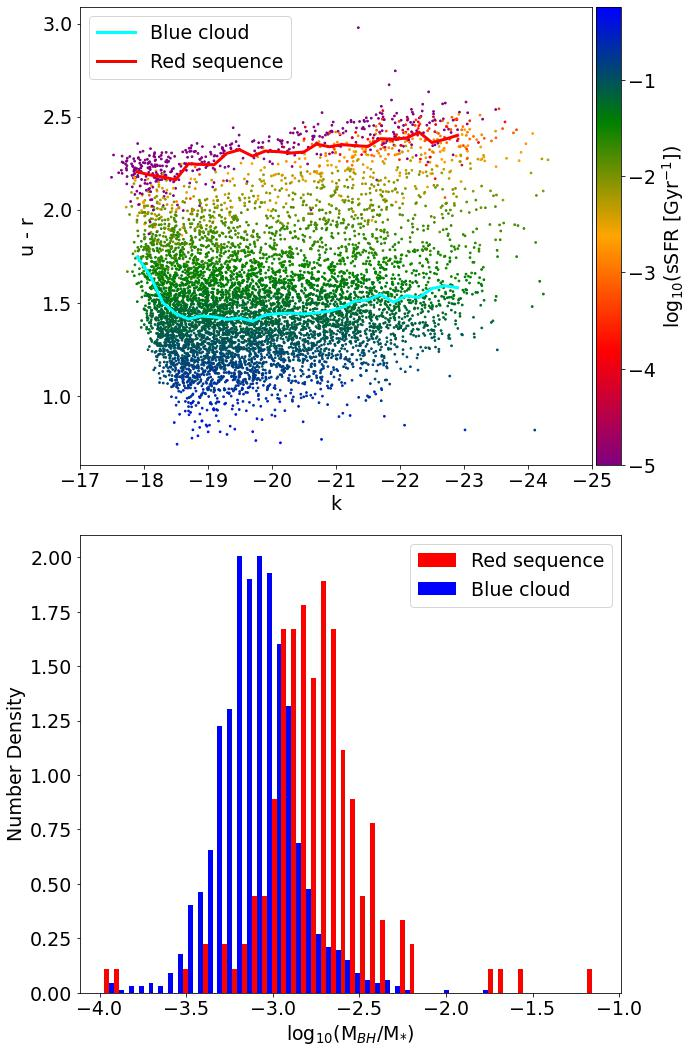
\includegraphics[width=11cm]{Plot_1.jpeg}
\caption{Top: u-r magnitude as a function of stellar mass for galaxies of mass greater than $10^9M_\odot$ at z=0. Individual galaxies are plotted as points, coloured by sSFR, using the colourbar to the right. Middle: Histogram of sSFR for galaxies of stellar mass between $10^{10} - 10^{10.5}M_\odot$ (the shaded region on the above plot). Bottom: Histogram of $M_{BH}/M_*$ for galaxies of stellar mass between $10^{10} - 10^{10.5}M_\odot$.}
\label{fig:1}
\end{figure}
\twocolumngrid


\noindent cloud galaxies is regulated by  stellar feedback, in which the energy injected into the interstellar medium by supernovae balances the energy lost due to cosmological accretion \cite{Ikea}. However, for galaxies more massive than a critical mass scale \cite{Quasar},

\begin{equation}
    M_{crit}\sim10^{12}\Delta_{z}^{-\frac{3}{8}}M_\odot
\end{equation}

\noindent where,

\begin{equation}
    \Delta_z\equiv(\Omega_m(1+z)^3+\Omega_\Lambda)^{\frac{1}{3}}
\end{equation}

\noindent outflows driven by supernovae will no longer be buoyant, leading to a buildup of gas in the central regions of the galaxy. This allows the central BH to grow rapidly, quickly reaching sufficient mass to begin AGN feedback, in which energy released by the BH heats the gas corona surrounding the galaxy, disrupting the inflow of cold gas and supressing star formation. More evidence of this can be seen from the colour of the points in Fig.2, as this shows a decrease in sSFR for galaxies with high BH mass and halo mass.

\section{Relating Halo mass to the Formation Rate of Quasars}

It can be seen from the right plot of Fig.2 that median BH mass increases exponentially for $11.75 \lesssim log_{10}(M_H) \lesssim 12.10$, equivalent to the rapid growth phase described in section 2. However, the total mass of the BH is still comparatively low during this phase, and so the BH cannot be considered to be luminous enough to be a quasar (qso) until it starts following the power law fit at $log_{10}(M_H) \gtrsim 12.10$. If we assume that the qso phase begins when $M_{BH}=M_{BH,start}=10^{7.5}M_\odot$ and ends when $M_{BH}=M_{BH,end}=10^8M_\odot$ (the region between the horizontal lines on Fig.2), then galaxies of halo mass between the vertical lines on Fig.2 can be assumed to contain

\onecolumngrid


\begin{figure}[H]
\centering
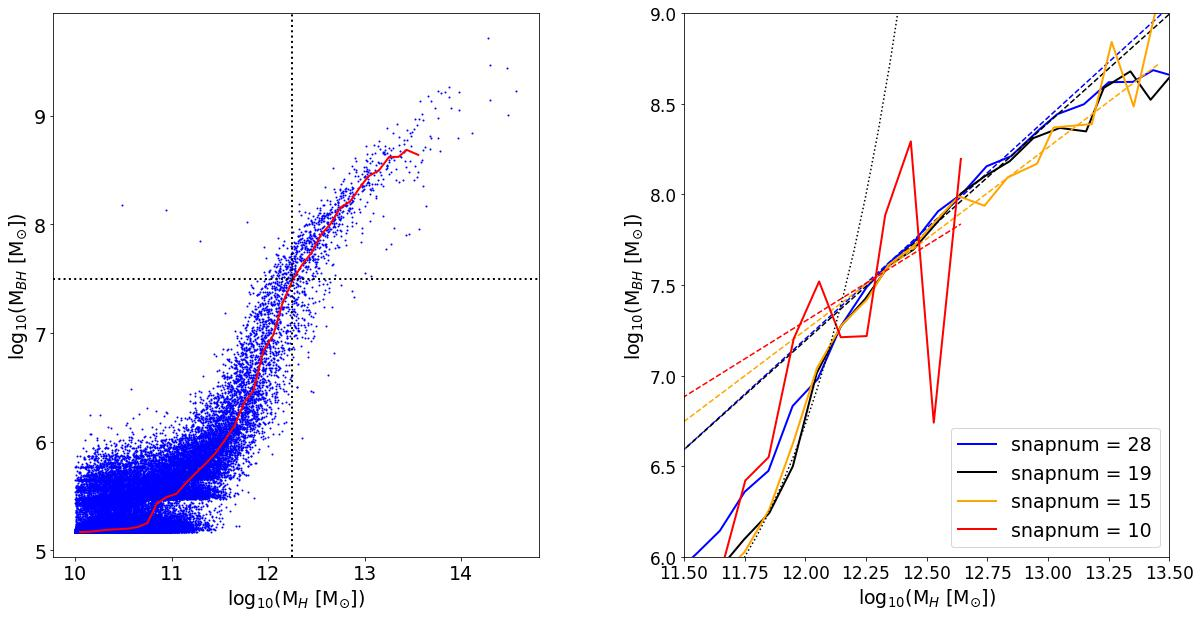
\includegraphics[width=17cm]{Plot_3.jpeg}
\caption{Left: Black hole mass - halo mass relation for central galaxies at z=0, the blue line shows median black hole mass. Individual galaxies are plotted as points, coloured by sSFR, using the colourbar to the right. Right: Median black hole mass as a function of halo mass for central galaxies at snapnums 28, 19, 15, and 10 (equivalent to z = 0, 1, 2, and 4 respectively). Dashed lines show power law fits, the dotted line shows an exponential fit.}
\label{fig:2}
\end{figure}
\twocolumngrid


\noindent quasars.\par

This means that the rate at which quasars are formed in EAGLE is equal to the rate at which galaxies cross the $10^{12}M_\odot$ halo mass threshold: $dn/dz$, where n is the number of galaxies of halo mass greater than $10^{12}M_\odot$ per unit comoving volume. This can be calculated using

\begin{equation}
    \frac{dn}{dz}=\frac{dn}{dln(M_H)}\frac{dln(M_H)}{dz}
\end{equation}

\noindent where $dn/dln(M_H)$ is the galaxy halo mass function for $M_H=10^{12}M_\odot$ at a given redshift, and the logarithmic growth rate is given by

\begin{equation}
    \frac{dln(M_H)}{dz}=\frac{a}{(1+z)}-b
\end{equation}

\noindent This corresponds to the parametrisation given in Sharma \& Theuns (2020) in which $M_H$ can be written as

\begin{align}
    \frac{M_H}{M_{H,0}}&=m_H(z) \nonumber \\
    m_H(z)&\approx(1+z)^ae^{-bz}
\end{align}

\noindent where a and b are fitting parameters, and $M_{H,0}$ is the value of $M_H$ at z=0. Sharma \& Theuns (2020) Gives values for a \& b, averaged over halo masses, as $\bar a \approx 0.24, \bar b \approx 0.75$, but to test their fit for the evolution of EAGLE galaxies crossing the $10^{12}M_\odot$ halo mass threshold, $M_H/M_{H,0}$ is plotted against z in Fig.3 for EAGLE galaxies and for $m_H(z)$. Fig.3 shows that Equation (5) fits the evolution of halo mass with redshift well for EAGLE galaxies crossing the $10^{12}M_\odot$ halo mass threshold. The outliers in Fig.3 that are significantly more massive than they are at z=0 are believed to be caused by halos passing through one another and contributing to each others' measured masses, before moving away at $z\approx0$, leading to  sudden decreases in the measured value of $M_H$.

\onecolumngrid


\begin{figure}[H]
\centering
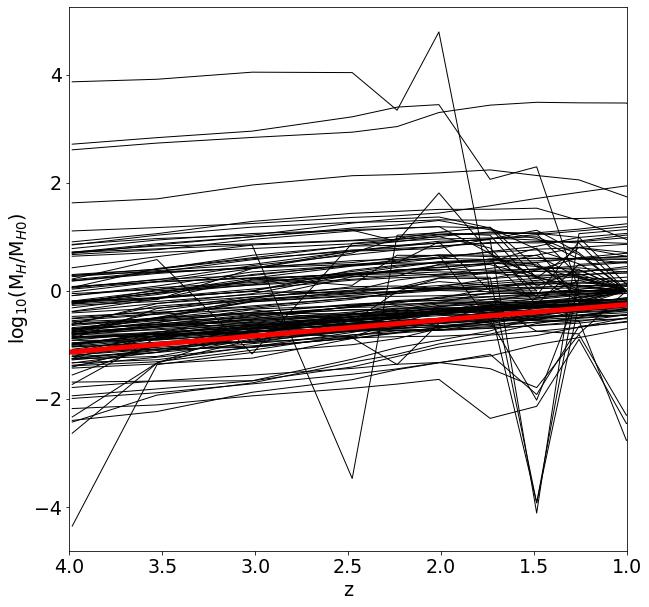
\includegraphics[width=\linewidth]{Plot_5.jpeg}
\caption{The black lines show $M_H/M_{H,0}$ as a function of redshift for central galaxies which cross the $10^{12}M_\odot$ halo mass threshold at z=2. The red line shows $M_H/M_{H,0}$ as described by Equation (5).}
\label{fig:3}
\end{figure}
\twocolumngrid


\section{Images}


\onecolumngrid


\begin{figure}[H]
\centering
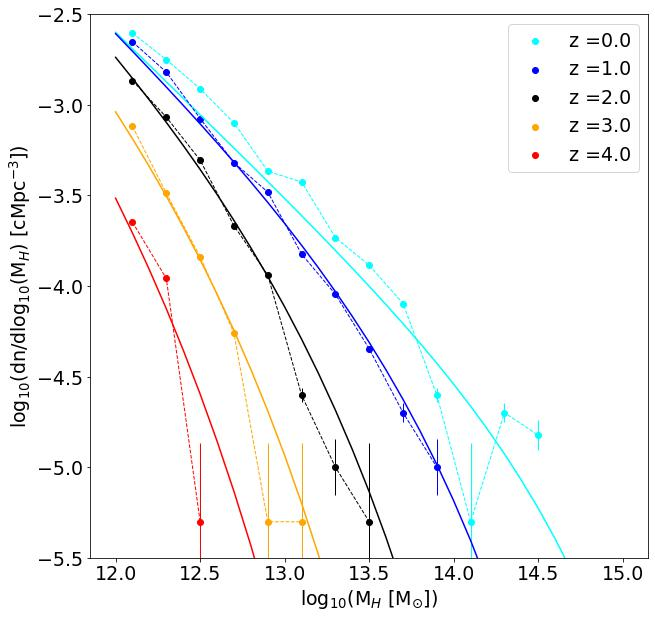
\includegraphics[width=\linewidth]{Mass_Function.jpeg}
\caption{Galaxy halo mass functions for galaxies of halo mass greater than $10^{12}M_\odot$ between z=0 and z=4. The dashed lines show mass functions from EAGLE, filled lines show mass functions from COLOSSUS.}
\label{fig:5}
\end{figure}
\twocolumngrid


\onecolumngrid


\begin{figure}[H]
\centering
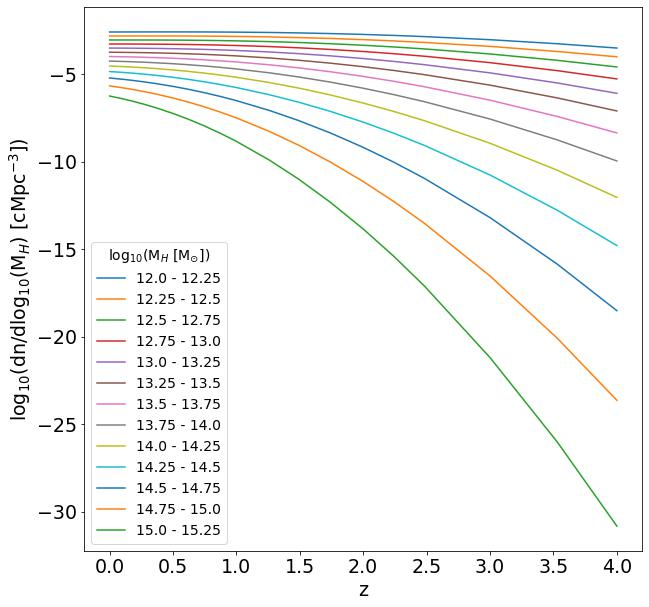
\includegraphics[width=\linewidth]{Mass_Function_2.jpeg}
\caption{Galaxy halo mass function as a function of redshift for galaxies of halo mass greater than $10^{12}M_\odot$. Produced using COLOSSUS.}
\label{fig:6}
\end{figure}
\twocolumngrid


\onecolumngrid


\begin{figure}[H]
\centering
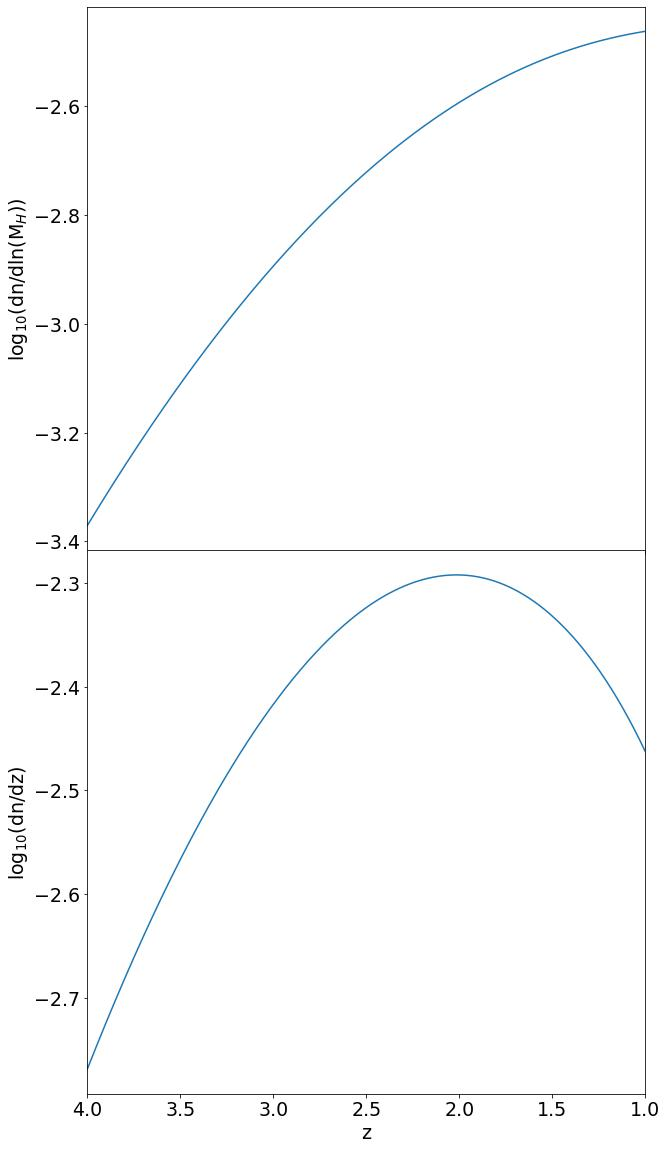
\includegraphics[width=12cm]{Plot_6.jpeg}
\caption{Top: Galaxy halo mass function as a function of redshift for galaxies of mass $10^{12}M_\odot$ produced using COLOSSUS. Bottom: Formation rate of halos of mass greater than $10^{12}M_\odot$ as a function of redshift, calculated using Equation (4). This appears to peak at z=2.}
\label{fig:8}
\end{figure}
\twocolumngrid


\section{Section heading}

Duis eget tellus tortor. Cum sociis natoque penatibus et magnis dis parturient montes, nascetur ridiculus mus. In tellus nulla, sodales eu pulvinar at, accumsan quis magna. Nunc sed lacus diam. Nam enim mauris, imperdiet ut egestas quis, tincidunt at odio. Ut viverra nulla at libero dictum aliquet. Suspendisse lacus lacus, imperdiet nec elit nec, ullamcorper facilisis ex. \cite{Ikea} \cite{EAGLE}

\subsection{Subsection heading}

Proin sit amet mauris tincidunt, consectetur nisi ultrices, dapibus elit. Nullam vitae faucibus odio, pharetra ultrices tortor. Class aptent taciti sociosqu ad litora torquent per conubia nostra, per inceptos himenaeos. 

\section{Conclusions}
Donec finibus, tellus sit amet luctus sodales, lectus ante accumsan ligula, at condimentum lorem justo a sapien. Phasellus vel tortor vitae metus lacinia efficitur ac vel ex. Aenean eget congue leo. Aliquam cursus mauris sit amet arcu dignissim, vel condimentum nisi sodales. 

\bibliographystyle{unsrtnat}
\bibliography{citation.bib}

\end{document}